%==============================================================
%  EE201 -- Circuit Theory I
%  Lecture 16 : Operational Amplifiers
%  M. Mert Ankaralı, METU EEE
%
%  Compile:  ./build.sh      (or: pdflatex EE201_Lecture_17.tex, twice)
%==============================================================
\documentclass[11pt,a4paper]{article}

%-------------------- packages --------------------------------
\usepackage[T1]{fontenc}
\usepackage[utf8]{inputenc}
\usepackage[english]{babel}
\usepackage{lmodern}
\usepackage[left=2.2cm,right=4.4cm,top=2.2cm,bottom=2.2cm,headheight=14pt,headsep=9pt,marginparwidth=3.4cm,marginparsep=0.5cm]{geometry}
\usepackage{amsmath,amssymb}
\usepackage{array,booktabs,tabularx}
\usepackage{enumitem}
\usepackage{needspace}
\usepackage[table]{xcolor}
\usepackage{fancyhdr}
\usepackage{titlesec}
\usepackage{graphicx}
\usepackage[most]{tcolorbox}
\usepackage{tikz}
\usepackage[american,siunitx]{circuitikz}
\usetikzlibrary{matrix,arrows.meta,positioning,calc,decorations.pathmorphing,decorations.pathreplacing,decorations.markings,patterns,shapes.geometric}
\usepackage[colorlinks=true,allcolors=metured,breaklinks=true]{hyperref}

%-------------------- colour system ---------------------------
% One colour per physical quantity, used identically in the slides.
\definecolor{metured}{RGB}{155,27,48}    % headings, structure
\definecolor{metugray}{RGB}{88,89,91}
\definecolor{ccur}{RGB}{0,102,170}       % CURRENT  -- blue
\definecolor{cvolt}{RGB}{214,120,0}      % VOLTAGE  -- orange
\definecolor{cpow}{RGB}{23,128,74}       % POWER / ENERGY -- green
\definecolor{ccharge}{RGB}{124,60,160}   % CHARGE   -- purple
\definecolor{cflux}{RGB}{0,138,138}      % FLUX -- teal
\definecolor{boxgray}{RGB}{245,245,245}
\definecolor{copper}{RGB}{184,98,30}

\newcommand{\Icol}[1]{\textcolor{ccur}{#1}}
\newcommand{\Vcol}[1]{\textcolor{cvolt}{#1}}
\newcommand{\Pcol}[1]{\textcolor{cpow}{#1}}
\newcommand{\Qcol}[1]{\textcolor{ccharge}{#1}}
\newcommand{\Fcol}[1]{\textcolor{cflux}{#1}}

%-------------------- units (no siunitx dependency) -----------
\newcommand{\uni}[1]{\,\mathrm{#1}}
\newcommand{\A}{\uni{A}}   \newcommand{\V}{\uni{V}}
\newcommand{\W}{\uni{W}}   \newcommand{\J}{\uni{J}}
\newcommand{\Cb}{\uni{C}}  \newcommand{\s}{\uni{s}}
\newcommand{\Sie}{\uni{S}} \newcommand{\Wb}{\uni{Wb}}

%-------------------- layout ----------------------------------
\pagestyle{fancy}
\fancyhf{}
\lhead{\small\textcolor{metugray}{EE201 -- Circuit Theory I}}
\rhead{\small\textcolor{metugray}{Lecture 16: Operational Amplifiers}}
\cfoot{\small\thepage}
\renewcommand{\headrulewidth}{0.4pt}

\titleformat{\section}{\large\bfseries\color{metured}}{\thesection.}{0.6em}{}
\titleformat{\subsection}{\normalsize\bfseries\color{metugray}}{\thesubsection.}{0.6em}{}
\titlespacing*{\section}{0pt}{1.4ex plus .3ex}{0.7ex}
\titlespacing*{\subsection}{0pt}{1.1ex plus .2ex}{0.5ex}

\setlist[itemize]{itemsep=2pt,topsep=3pt,parsep=0pt,leftmargin=1.5em}
\setlist[enumerate]{itemsep=2pt,topsep=3pt,parsep=0pt,leftmargin=1.7em}
\setlength{\parindent}{0pt}
\setlength{\parskip}{1.2ex plus .2ex}
\linespread{1.25}
\AtBeginDocument{\setlength{\abovedisplayskip}{12pt plus 3pt}\setlength{\belowdisplayskip}{12pt plus 3pt}}
\raggedbottom
\widowpenalty=10000
\clubpenalty=10000
\brokenpenalty=10000

%-------------------- boxes -----------------------------------
\newtcolorbox{definitionbox}[1]{enhanced,
  colback=metured!4, colframe=metured, boxrule=0.9pt,
  fonttitle=\bfseries, title={#1}, arc=2pt,
  left=7pt,right=7pt,top=5pt,bottom=5pt, before skip=7pt, after skip=7pt,
  before upper={\setlength{\parskip}{0.6ex plus .1ex}}}

\newtcolorbox{ideabox}[1][Key idea]{enhanced,
  colback=ccur!5, colframe=ccur, boxrule=0.9pt,
  fonttitle=\bfseries, title={#1}, arc=2pt,
  left=7pt,right=7pt,top=5pt,bottom=5pt, before skip=7pt, after skip=7pt,
  before upper={\setlength{\parskip}{0.6ex plus .1ex}}}

\newtcolorbox{examplebox}[1][Example]{enhanced,
  colback=cpow!4, colframe=cpow, boxrule=0.9pt,
  fonttitle=\bfseries, title={#1}, arc=2pt,
  left=7pt,right=7pt,top=5pt,bottom=5pt, before skip=7pt, after skip=7pt,
  before upper={\setlength{\parskip}{0.6ex plus .1ex}}}

%  Example solutions: a heading and numbered steps outside the example box
\newif\ifsolfirst
\newcommand{\solution}{\par\smallskip\noindent{\color{cpow}\bfseries Solution}\par\nobreak\smallskip\global\solfirsttrue}
\newcommand{\solstep}[2]{\par\ifsolfirst\global\solfirstfalse\else\bigskip\needspace{5\baselineskip}\fi
  \noindent{\color{cpow}\bfseries Step #1.}\ {\bfseries #2}\par\nobreak\smallskip}

\newtcolorbox{cautionbox}[1][Careful]{enhanced,
  colback=cvolt!6, colframe=cvolt, boxrule=0.9pt,
  fonttitle=\bfseries, title={#1}, arc=2pt,
  left=7pt,right=7pt,top=5pt,bottom=5pt, before skip=7pt, after skip=7pt,
  before upper={\setlength{\parskip}{0.6ex plus .1ex}}}

%-------------------- circuitikz defaults ---------------------
%  voltage sources: smaller + and - inside the circle, further apart
\ctikzset{bipoles/vsourceam/inner plus={\tiny$+$},
          bipoles/vsourceam/inner minus={\tiny$\vphantom{+}-$},
          bipoles/vsourceam/margin=0.85,
          bipoles/cvsourceam/inner plus={\tiny$+$},
          bipoles/cvsourceam/inner minus={\tiny$\vphantom{+}-$},
          bipoles/cvsourceam/margin=0.85}
\ctikzset{bipoles/length=0.9cm, color=black,
          label/align=straight,
          bipoles/generic/height=0.28, bipoles/generic/width=0.62}
\tikzset{
  iar/.style={-{Stealth[length=2.2mm]}, ccur, thick},
  pol/.style={font=\small, text=cvolt},
  glab/.style={font=\footnotesize, text=metured},
  ttl/.style={font=\scriptsize\bfseries, text=metugray},
  capn/.style={font=\scriptsize, text=metugray, align=center},
  bigarr/.style={-{Stealth[length=3mm]}, very thick, metugray},
  gnode/.style={circle, fill=metured, inner sep=0pt, minimum size=4.4pt},
  nlab/.style={circle, draw=metured, text=metured, font=\scriptsize, inner sep=0.7pt},
  blab/.style={font=\footnotesize, text=black!80},
  gbr/.style={black!75, thick, postaction={decorate, decoration={markings,
      mark=at position 0.56 with {\arrow{Stealth[length=2.5mm]}}}}},
  apbr/.style={ccur, line width=1.7pt, postaction={decorate, decoration={markings,
      mark=at position 0.56 with {\arrow{Stealth[length=2.8mm]}}}}},
  hal/.style={draw=cpow!60, line width=6pt, opacity=0.35, line cap=round, line join=round},
  elem/.style={draw=metugray, thick, fill=metulight},
}
\definecolor{metulight}{RGB}{243,240,241}

%-------------------- Lecture 16-17 macros: operational amplifiers ---------------
\newcommand{\ohm}{\,\Omega}
\newcommand{\kohm}{\,\mathrm{k}\Omega}
\newcommand{\mA}{\,\mathrm{mA}}
\newcommand{\mF}{\,\mathrm{mF}}
\newcommand{\yes}{\textcolor{cpow}{\checkmark}}
\newcommand{\vin}{\Vcol{v_{\mathrm{in}}}}
\newcommand{\vo}{\Vcol{v_o}}
\newcommand{\vp}{\Vcol{v_+}}
\newcommand{\vm}{\Vcol{v_-}}
\newcommand{\ip}{\Icol{i_+}}
\newcommand{\im}{\Icol{i_-}}
\newcommand{\Es}{E_s}
\newcommand{\lR}[3]{\node[anchor=west, xshift=7pt, font=\small] at (#1,#2) {#3};}
\newcommand{\lL}[3]{\node[anchor=east, xshift=-7pt, font=\small] at (#1,#2) {#3};}
\tikzset{vax/.style={-{Stealth[length=2mm]}, gray!70},
         crv/.style={metured, very thick, line join=round},
         crvu/.style={metured, very thick, dashed, line join=round},
         gdash/.style={black!45, densely dashed, thin},
         oa/.style={op amp, fill=metulight, thick},
         reg/.style={font=\scriptsize, text=metugray, align=center}}

%  ---------- the device ----------
%  op-amp with labels of all terminals and the supplies
\newcommand{\oaDevice}{%
  \node[oa] (A) at (0,0) {};
  \draw (A.-) -- ++(-0.6,0) node[ocirc] {} node[left, font=\small] {inverting ($-$)};
  \draw (A.+) -- ++(-0.6,0) node[ocirc] {} node[left, font=\small] {non-inverting ($+$)};
  \draw (A.out) -- ++(0.7,0) node[ocirc] {} node[right, font=\small] {output};
  \draw (A.up) -- ++(0,0.5) node[above, font=\small] {$E_+$};
  \draw (A.down) -- ++(0,-0.5) node[below, font=\small] {$E_-$};}
%  terminal voltages w.r.t. the common ground
\newcommand{\oaVolt}{%
  \node[oa] (A) at (0,0) {};
  \draw (A.-) -- ++(-0.7,0) node[ocirc] (m) {}; \draw (A.+) -- ++(-0.7,0) node[ocirc] (p) {};
  \draw (A.out) -- ++(0.8,0) node[ocirc] (o) {};
  \draw[iar] ($(m)+(0.15,0.2)$) -- ++(0.4,0); \node[font=\small, text=ccur, above] at ($(m)+(0.35,0.2)$) {$i_-$};
  \draw[iar] ($(p)+(0.15,-0.2)$) -- ++(0.4,0); \node[font=\small, text=ccur, below] at ($(p)+(0.35,-0.2)$) {$i_+$};
  \draw[iar] ($(o)+(-0.15,0.22)$) -- ++(-0.4,0); \node[font=\small, text=ccur, above] at ($(o)+(-0.35,0.22)$) {$i_o$};
  \node[font=\small, text=cvolt, left] at (m) {$v_-$}; \node[font=\small, text=cvolt, left] at (p) {$v_+$};
  \node[font=\small, text=cvolt, right] at (o) {$v_o$};
  \draw (A.down) -- ++(0,-0.35) node[ground] {};}
%  transfer characteristic v_o versus v_d = v_+ - v_-  (#1 = 1: with region names)
\newcommand{\oaChar}[1]{%
  \draw[vax] (-2.8,0) -- (2.9,0) node[right, font=\small] {$\Vcol{v_+ - v_-}$};
  \draw[vax] (0,-1.7) -- (0,1.8) node[above, font=\small] {$\vo$};
  \draw[gdash] (-0.6,-1.2) -- (-0.6,0); \draw[gdash] (0.6,1.2) -- (0.6,0);
  \draw[gdash] (0,1.2) -- (0.6,1.2); \draw[gdash] (0,-1.2) -- (-0.6,-1.2);
  \draw[crv] (-2.6,-1.2) -- (-0.6,-1.2) -- (0.6,1.2) -- (2.6,1.2);
  \node[font=\small, left] at (0,1.2) {$\Es$}; \node[font=\small, right] at (0,-1.2) {$-\Es$};
  \node[font=\scriptsize, anchor=west] at (0.45,0.55) {slope $A$};
  \ifnum#1=1
    \draw[|<->|, metugray] (-2.6,-2.0) -- (-0.6,-2.0) node[midway, below, reg] {$-$sat};
    \draw[|<->|, metugray] (-0.6,-2.0) -- (0.6,-2.0) node[midway, below, reg] {linear};
    \draw[|<->|, metugray] (0.6,-2.0) -- (2.6,-2.0) node[midway, below, reg] {$+$sat};
  \fi}
%  ideal (A -> infinity) characteristic
\newcommand{\oaIdealChar}{%
  \draw[vax] (-2.4,0) -- (2.5,0) node[right, font=\small] {$\Vcol{v_+ - v_-}$};
  \draw[vax] (0,-1.7) -- (0,1.8) node[above, font=\small] {$\vo$};
  \draw[crv] (-2.2,-1.2) -- (0,-1.2) -- (0,1.2) -- (2.2,1.2);
  \node[font=\small, left] at (0,1.45) {$\Es$}; \node[font=\small, right] at (0,-1.45) {$-\Es$};
  \node[reg, above] at (1.4,1.2) {$+$sat}; \node[reg, below] at (-1.4,-1.2) {$-$sat};
  \node[reg, anchor=west] at (0.05,0.45) {linear};}
%  dependent-source model in the linear region
\newcommand{\oaModel}{%
  \draw (0,1.6) node[ocirc] {} node[left, font=\small, text=cvolt] {$v_+$} -- (0.8,1.6) to[R, l_=$R_{\mathrm{in}}$] (0.8,0) -- (0,0) node[ocirc] {} node[left, font=\small, text=cvolt] {$v_-$};
  \draw (3.0,1.6) to[american controlled voltage source, l=$A(\Vcol{v_+ - v_-})$] (3.0,-0.6);
  \draw (3.0,1.6) to[R, l=$R_o$] (4.8,1.6) node[ocirc] {} node[right, font=\small, text=cvolt] {$v_o$};
  \draw (3.0,-0.6) node[ground] {};}

%  ---------- basic circuits (op-amp centred at (0,0)) ----------
%  voltage follower: #1 = 0 negative feedback, 1 positive feedback (inputs swapped)
\newcommand{\follower}[1]{%
  \ifnum#1=0 \node[oa, noinv input up] (A) at (0,0) {}; \else \node[oa] (A) at (0,0) {}; \fi
  \ifnum#1=0
    \draw (A.+) -- ++(-1.4,0) node[ocirc] {} node[left, font=\small, text=cvolt] {$v_{\mathrm{in}}$};
    \draw (A.-) -- ++(-0.4,0) -- ++(0,-0.9) -| (1.6,0) (A.out) -- (2.2,0) node[ocirc] {} node[right, font=\small, text=cvolt] {$v_o$};
  \else
    \draw (A.-) -- ++(-1.4,0) node[ocirc] {} node[left, font=\small, text=cvolt] {$v_{\mathrm{in}}$};
    \draw (A.+) -- ++(-0.4,0) -- ++(0,-0.9) -| (1.6,0) (A.out) -- (2.2,0) node[ocirc] {} node[right, font=\small, text=cvolt] {$v_o$};
  \fi
  \fill (1.6,0) circle (1.6pt);}
%  inverting amplifier with labels #1 (R_1), #2 (R_f), #3 (v_in)
\newcommand{\invAmp}[3]{%
  \node[oa] (A) at (0,0) {};
  \draw (A.-) -- ++(-0.4,0) coordinate (n) to[R, l_=#1] ++(-2.0,0) coordinate (s);
  \draw (s) to[american voltage source, l_=#3] ($(s)+(0,-1.8)$) node[ground] {};
  \draw (n) -- ++(0,1.3) coordinate (f) to[R, l=#2] (f -| A.out) -- (A.out);
  \draw (A.+) -- ++(-0.4,0) -- ++(0,-0.4) node[ground] {};
  \draw (A.out) -- ++(0.8,0) node[ocirc] {} node[right, font=\small, text=cvolt] {$v_o$};
  \fill (n) circle (1.6pt); \fill (A.out) circle (1.6pt);}
%  non-inverting amplifier with labels #1 (R_1), #2 (R_f), #3 (v_in)
\newcommand{\noninvAmp}[3]{%
  \node[oa] (A) at (0,0) {};
  \draw (A.-) -- ++(-1.6,0) coordinate (n) to[R, l_=#1] ++(0,-2.5) node[ground] {};
  \draw (A.+) -- ++(-0.6,0) coordinate (s) to[american voltage source, l=#3] ($(s)+(0,-1.6)$) node[ground] {};
  \draw (n) -- ++(0,1.3) coordinate (f) to[R, l=#2] (f -| A.out) -- (A.out);
  \draw (A.out) -- ++(0.8,0) node[ocirc] {} node[right, font=\small, text=cvolt] {$v_o$};
  \fill (n) circle (1.6pt); \fill (A.out) circle (1.6pt);}
%  summing amplifier with two inputs: #1 (R_1), #2 (R_2), #3 (R_f)
\newcommand{\summing}[3]{%
  \node[oa] (A) at (0,0) {};
  \draw (A.-) -- ++(-0.6,0) coordinate (n);
  \draw (n) to[R, l_=#1] ++(-2.2,0) node[ocirc] {} node[left, font=\small, text=cvolt] {$v_1$};
  \draw (n) -- ++(0,-1.2) coordinate (n2) to[R, l=#2] ++(-2.2,0) node[ocirc] {} node[left, font=\small, text=cvolt] {$v_2$};
  \draw (n) -- ++(0,1.2) coordinate (f) to[R, l=#3] (f -| A.out) -- (A.out);
  \draw (A.+) -- ++(-0.3,0) -- ++(0,-0.3) node[ground] {};
  \draw (A.out) -- ++(0.8,0) node[ocirc] {} node[right, font=\small, text=cvolt] {$v_o$};
  \fill (n) circle (1.6pt); \fill (A.out) circle (1.6pt);}
%  difference amplifier: #1 R_1, #2 R_2, #3 R_3, #4 R_f
\newcommand{\difference}[4]{%
  \node[oa] (A) at (0,0) {};
  \draw (A.-) -- ++(-0.6,0) coordinate (n) to[R, l_=#1] ++(-2.0,0) node[ocirc] {} node[left, font=\small, text=cvolt] {$v_1$};
  \draw (A.+) -- ++(-0.6,0) coordinate (q) to[R, l=#2] ++(-2.0,0) node[ocirc] {} node[left, font=\small, text=cvolt] {$v_2$};
  \draw (q) to[R, l=#3] ++(0,-1.6) node[ground] {};
  \draw (n) -- ++(0,1.3) coordinate (f) to[R, l=#4] (f -| A.out) -- (A.out);
  \draw (A.out) -- ++(0.8,0) node[ocirc] {} node[right, font=\small, text=cvolt] {$v_o$};
  \fill (n) circle (1.6pt); \fill (q) circle (1.6pt); \fill (A.out) circle (1.6pt);}
%  integrator (#1 = 0) or differentiator (#1 = 1): input element and feedback element
\newcommand{\intdiff}[1]{%
  \node[oa] (A) at (0,0) {};
  \ifnum#1=0
    \draw (A.-) -- ++(-0.4,0) coordinate (n) to[R, l_=$R$] ++(-2.0,0) coordinate (s);
    \draw (n) -- ++(0,1.3) coordinate (f) to[C, l_=$C$] (f -| A.out) -- (A.out);
    \node[pol] at ($(f)+(0.45,0.38)$) {$+$}; \node[pol] at ($(f -| A.out)+(-0.45,0.38)$) {$-$};
    \node[font=\small, text=cvolt] at ($(f)!0.5!(f -| A.out)+(0,0.45)$) {$v_C$};
    \draw[iar] ($(s)+(0.35,0.28)$) -- ++(0.5,0); \node[font=\small, text=ccur, above] at ($(s)+(0.6,0.28)$) {$i$};
  \else
    \draw (A.-) -- ++(-0.4,0) coordinate (n) to[C, l_=$C$] ++(-2.0,0) coordinate (s);
    \draw (n) -- ++(0,1.3) coordinate (f) to[R, l=$R$] (f -| A.out) -- (A.out);
    \node[pol] at ($(s)+(0.35,0.42)$) {$+$}; \node[pol] at ($(n)+(-0.35,0.42)$) {$-$};
    \draw[iar] ($(f)+(0.3,0.32)$) -- ++(0.5,0); \node[font=\small, text=ccur, above] at ($(f)+(0.55,0.32)$) {$i$};
  \fi
  \draw (s) to[american voltage source, l_=$\Vcol{v_{\mathrm{in}}}$] ($(s)+(0,-1.8)$) node[ground] {};
  \draw (A.+) -- ++(-0.4,0) -- ++(0,-0.4) node[ground] {};
  \draw (A.out) -- ++(0.8,0) node[ocirc] {} node[right, font=\small, text=cvolt] {$v_o$};
  \fill (n) circle (1.6pt); \fill (A.out) circle (1.6pt);}
%  buffer example: 12 V, 2k / 1k divider, 2k load. #1 = 0 load directly, 1 through a buffer
\newcommand{\bufEx}[1]{%
  \draw (0,0) to[american voltage source, l=$\Vcol{12\V}$, invert] (0,2.2) to[R, l=$2\kohm$] (2.2,2.2) to[R, l_=$1\kohm$, *-] (2.2,0) -- (0,0);
  \ifnum#1=0
    \draw (2.2,2.2) -- (4.0,2.2) to[R, l=$2\kohm$] (4.0,0) -- (2.2,0);
    \node[font=\small, text=cvolt] at (3.1,1.1) {$v$};
    \node[pol] at (3.1,1.6) {$+$}; \node[pol] at (3.1,0.6) {$-$};
  \else
    \node[oa, noinv input up, anchor=+] (B) at (3.9,2.2) {};
    \draw (2.2,2.2) -- (B.+); \fill (2.2,2.2) circle (1.6pt);
    \draw (B.out) -- ++(0.9,0) coordinate (fo) -- ++(1.6,0) coordinate (lo);
    \draw (B.-) -- ++(-0.4,0) -- ++(0,-0.8) -| (fo);
    \draw (lo) to[R, l_=$2\kohm$] (lo |- 0,0) node[ground] {};
    \fill (fo) circle (1.6pt);
    \node[font=\small, text=cvolt] at ($(lo |- 0,1.0)+(0.6,0)$) {$v$};
    \node[pol] at ($(lo |- 0,1.5)+(0.6,0)$) {$+$}; \node[pol] at ($(lo |- 0,0.5)+(0.6,0)$) {$-$};
  \fi
  \draw (0,0) node[ground] {};}
%  axes and ticks for transfer characteristics drawn in data units
\newcommand{\tax}[6]{\draw[vax] (#1,0) -- (#2,0) node[right, font=\small] {#5};
  \draw[vax] (0,#3) -- (0,#4) node[above, font=\small] {#6};}
\newcommand{\xt}[2]{\draw ([yshift=2pt]#1,0) -- ([yshift=-2pt]#1,0) node[below, font=\scriptsize] {#2};}
\newcommand{\xtu}[2]{\draw ([yshift=2pt]#1,0) -- ([yshift=-2pt]#1,0); \node[above, font=\scriptsize] at (#1,0) {#2};}
\newcommand{\yt}[2]{\draw ([xshift=2pt]0,#1) -- ([xshift=-2pt]0,#1) node[left, font=\scriptsize] {#2};}
\newcommand{\ytr}[2]{\draw ([xshift=2pt]0,#1) -- ([xshift=-2pt]0,#1); \node[right, font=\scriptsize] at (0,#1) {#2};}

%  ---------- Lecture 17 circuits ----------
%  two feedback paths: #1 R_1, #2 R_2, #3 R_3, #4 R_4
\newcommand{\twoFb}[4]{%
  \node[oa] (A) at (0,0) {};
  \draw (A.-) -- ++(-0.4,0) coordinate (n) to[R, l_=#1] ++(-2.6,0) coordinate (s);
  \draw (s) to[american voltage source, l_=$\Vcol{v_{\mathrm{in}}}$] ($(s)+(0,-1.8)$) node[ground] {};
  \draw[iar] ($(s)+(0.25,0.25)$) -- ++(0.5,0); \node[font=\small, text=ccur, anchor=east] at ($(s)+(0.25,0.3)$) {$i$};
  \draw (n) -- ++(0,1.3) coordinate (f) to[R, l=#2] (f -| A.out) -- (A.out);
  \draw (A.+) -- ++(-0.4,0) coordinate (q) -- ++(0,-1.0) coordinate (b) to[R, l_=#4] (b -| A.out) -- (A.out);
  \draw (q) -- ++(-1.0,0) coordinate (g) to[R, l_=#3] ++(0,-1.6) node[ground] {};
  \draw (A.out) -- ++(0.8,0) node[ocirc] {} node[right, font=\small, text=cvolt] {$v_o$};
  \fill (n) circle (1.6pt); \fill (q) circle (1.6pt); \fill (A.out) circle (1.6pt);}
%  numerical positive-feedback circuit (Example 17.4)
\newcommand{\numPF}{%
  \node[oa] (A) at (0,0) {};
  \draw (A.-) -- ++(-2.8,0) coordinate (a);
  \draw (a) -- ++(0,1.3) coordinate (f) to[R, l=$2\kohm$] (f -| A.out) -- (A.out);
  \draw (a) |- ($(A.+)+(-2.8,0)$) to[R, l_=$1\kohm$] ($(A.+)+(-0.5,0)$) coordinate (q) -- (A.+);
  \draw (q) -- ++(0,-0.9) coordinate (r) to[R, l_=$2\kohm$] (r -| A.out) -- (A.out);
  \draw (r) to[R, l_=$2\kohm$] ++(0,-1.7) to[american voltage source, l_=$4\V$] ++(0,-1.6) node[ground] {};
  \draw (a) -- ++(-1.0,0) coordinate (s) to[american voltage source, l_=$\Vcol{v_{\mathrm{in}}}$] ($(s)+(0,-2.0)$) node[ground] {};
  \draw[iar] ($(s)+(0.2,0.28)$) -- ++(0.5,0); \node[font=\small, text=ccur, above] at ($(s)+(0.45,0.28)$) {$i$};
  \draw (A.out) -- ++(0.8,0) node[ocirc] {} node[right, font=\small, text=cvolt] {$v_o$};
  \fill (a) circle (1.6pt); \fill (q) circle (1.6pt); \fill (r) circle (1.6pt); \fill (A.out) circle (1.6pt);}
%  follower with the dependent-source model (finite gain)
\newcommand{\fgFollower}{%
  \draw (-1.4,1.6) to[american voltage source, l_=$\Vcol{v_s}$] (-1.4,0); \draw (-1.4,1.6) to[R, l=$R_s$] (1.2,1.6) coordinate (P);
  \draw (P) to[R, l=$R_{\mathrm{in}}$] (1.2,0) coordinate (M);
  \draw (3.2,1.6) to[american controlled voltage source, l=$A(\Vcol{v_+ - v_-})$] (3.2,0.2) node[ground] {};
  \draw (3.2,1.6) to[R, l=$R_o$] (7.0,1.6) coordinate (O);
  \draw (O) to[R, l=$R_L$] (7.0,0.2) node[ground] {};
  \draw (M) -- (1.2,-0.7) -- (7.8,-0.7) -- (7.8,1.6) -- (O);
  \draw (7.8,1.6) -- (8.3,1.6) node[ocirc] {} node[right, font=\small, text=cvolt] {$v_o$};
  \draw (-1.4,0) node[ground] {};
  \node[font=\small, text=cvolt, above left] at (P) {$v_+$}; \node[font=\small, text=cvolt, left] at (M) {$v_-$};
  \draw[iar] ($(P)+(-0.35,-0.3)$) -- ++(0,-0.5); \node[font=\small, text=ccur, left] at ($(P)+(-0.35,-0.55)$) {$i_+$};
  \fill (P) circle (1.6pt); \fill (M) circle (1.6pt); \fill (O) circle (1.6pt); \fill (7.8,1.6) circle (1.6pt);}
%  finite-gain ideal model: open inputs, ideal controlled source at the output
\newcommand{\oaFGModel}{%
  \draw (0,1.6) node[ocirc] {} node[left, font=\small, text=cvolt] {$v_+$} -- (0.5,1.6);
  \draw (0,0) node[ocirc] {} node[left, font=\small, text=cvolt] {$v_-$} -- (0.5,0);
  \node[font=\small, text=ccur] at (0.9,0.8) {$i_\pm = 0$};
  \draw (2.6,1.6) to[american controlled voltage source, l=$A(\Vcol{v_+ - v_-})$] (2.6,-0.6) node[ground] {};
  \draw (2.6,1.6) -- (3.6,1.6) node[ocirc] {} node[right, font=\small, text=cvolt] {$v_o$};}
%  negative-feedback loop: v_o too high -> v_- rises -> difference falls -> v_o down
\tikzset{cn/.style={circle, fill=metured, text=white, inner sep=0.6pt, minimum size=3.4mm, font=\scriptsize\bfseries}}
\newcommand{\cnum}[1]{\tikz[baseline=(cnumnode.base)]\node[cn] (cnumnode) {#1};}
\newcommand{\fbLoop}{%
  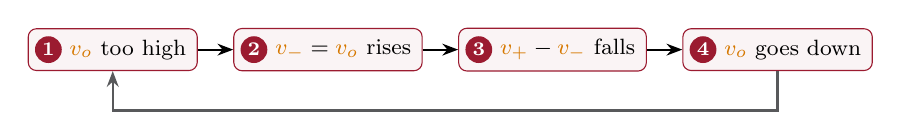
\begin{tikzpicture}[font=\footnotesize, st/.style={draw=metured, rounded corners=3pt, fill=metured!5, inner sep=4pt}]
    \node[st] (a) at (0,0) [label={[cn, label distance=-4.4mm]west:1}] {\hspace{11pt}$\vo$ too high};
    \node[st, anchor=west] (b) at ($(a.east)+(0.45,0)$) [label={[cn, label distance=-4.4mm]west:2}] {\hspace{11pt}$\vm = \vo$ rises};
    \node[st, anchor=west] (c) at ($(b.east)+(0.45,0)$) [label={[cn, label distance=-4.4mm]west:3}] {\hspace{11pt}$\vp - \vm$ falls};
    \node[st, anchor=west] (e) at ($(c.east)+(0.45,0)$) [label={[cn, label distance=-4.4mm]west:4}] {\hspace{11pt}$\vo$ goes down};
    \draw[-{Stealth[length=2mm]}, thick] (a) -- (b);
    \draw[-{Stealth[length=2mm]}, thick] (b) -- (c);
    \draw[-{Stealth[length=2mm]}, thick] (c) -- (e);
    \draw[-{Stealth[length=2mm]}, thick, metugray] (e.south) -- ++(0,-0.5) -| (a.south);
  \end{tikzpicture}}
%  block diagram of the follower: difference operator, op-amp block A, unity feedback
%  #1 = 1: show the numbered steps of the loop
\newcommand{\fbBlock}[1]{%
  \begin{tikzpicture}[font=\small, >={Stealth[length=2.2mm]}]
    \node[draw, circle, thick, minimum size=6.5mm, inner sep=0pt] (s) at (1.2,0) {};
    \node[font=\scriptsize] at ($(s)+(-0.45,0.22)$) {$+$};
    \node[font=\scriptsize] at ($(s)+(0.22,-0.48)$) {$-$};
    \node[draw, thick, fill=metulight, minimum width=1.2cm, minimum height=0.85cm] (b) at (3.4,0) {$A$};
    \node[font=\scriptsize, text=metugray, above] at (b.north) {op-amp};
    \draw[->, thick] (0,0) node[left, text=cvolt] {$v_{\mathrm{in}}$} -- (s.west);
    \draw[->, thick] (s.east) -- (b.west) node[midway, above, text=cvolt] {$v_d$};
    \draw[->, thick] (b.east) -- (5.6,0) node[right, text=cvolt] {$v_o$};
    \fill (4.8,0) circle (1.6pt);
    \draw[->, thick, metured] (4.8,0) -- (4.8,-1.3) -- (1.2,-1.3) -- (s.south);
    \node[font=\small, text=cvolt, anchor=east] at (1.12,-0.85) {$v_-$};
    \ifnum#1=1
      \node[cn] at (5.1,0.33) {1};
      \node[cn] at (1.5,-0.9) {2};
      \node[cn] at (2.4,-0.33) {3};
      \node[cn] at (4.25,0.62) {4};
    \fi
  \end{tikzpicture}}

%  source with internal resistance -> follower -> load, and its equivalent
\newcommand{\bufThev}{%
  \draw (0,1.8) to[american voltage source, l_=$\Vcol{v_s}$] (0,0) node[ground] {};
  \draw (0,1.8) to[R, l=$R_s$] (2.0,1.8) coordinate (p);
  \node[oa, noinv input up, anchor=+] (B) at (2.6,1.8) {};
  \draw (p) -- (B.+);
  \draw (B.out) -- ++(0.7,0) coordinate (fo) -- ++(1.2,0) coordinate (lo);
  \draw (B.-) -- ++(-0.4,0) -- ++(0,-0.8) -| (fo);
  \draw (lo) to[R, l_=$R_L$] (lo |- 0,0) node[ground] {};
  \fill (fo) circle (1.6pt);
  \draw[iar] (0.65,1.45) -- (1.3,1.45); \node[font=\small, text=ccur, below] at (0.97,1.45) {$i_+ = 0$};
  \node[font=\small, text=cvolt] at ($(lo |- 0,0.9)+(0.6,0)$) {$v_s$};
  \node[pol] at ($(lo |- 0,1.4)+(0.6,0)$) {$+$}; \node[pol] at ($(lo |- 0,0.4)+(0.6,0)$) {$-$};}
\newcommand{\bufEquiv}{%
  \draw (0,1.8) to[american voltage source, l_=$\Vcol{v_s}$] (0,0) node[ground] {};
  \draw (0,1.8) -- (1.6,1.8) to[R, l=$R_L$] (1.6,0) -- (0,0);}
%  KCL at the inverting input of an inverting amplifier: node v_- and its three currents
\newcommand{\kclFig}{%
  \node[oa] (A) at (0,0) {};
  \draw (A.-) -- ++(-1.3,0) coordinate (n) to[R, l_=$R_1$] ++(-2.3,0) coordinate (s);
  \draw (s) to[american voltage source, l_=$\Vcol{v_{\mathrm{in}}}$] ($(s)+(0,-1.9)$) node[ground] {};
  \draw (n) -- ++(0,1.8) coordinate (f) to[R, l=$R_f$] (f -| A.out) -- (A.out);
  \draw (A.+) -- ++(-0.5,0) -- ++(0,-0.45) node[ground] {};
  \draw (A.out) -- ++(0.8,0) node[ocirc] {} node[right, font=\small, text=cvolt] {$v_o$};
  \fill (A.out) circle (1.6pt);
  \draw[cvolt, thick, fill=cvolt!15] (n) circle (0.16);
  \node[font=\small, text=cvolt, anchor=north] at ($(n)+(0,-0.22)$) {$v_-$};
  \draw[iar] ($(n)+(-1.6,-0.35)$) -- ++(0.7,0); \node[font=\small, text=ccur, below] at ($(n)+(-1.25,-0.35)$) {$i_1$};
  \draw[iar] ($(f)+(0.6,-0.35)$) -- ++(0.7,0); \node[font=\small, text=ccur, below] at ($(f)+(0.95,-0.35)$) {$i_f$};
  \draw[iar] ($(n)+(0.4,0.25)$) -- ++(0.6,0); \node[font=\small, text=ccur, above] at ($(n)+(0.8,0.25)$) {$i_- = 0$};
  \node[font=\small, text=cvolt, anchor=west] at ($(A.+)+(-0.4,-0.75)$) {$v_+ = 0$};}
%  positive-feedback block diagram: v_in enters with a minus sign, the output returns with a plus sign
\newcommand{\fbBlockPos}[1]{%
  \begin{tikzpicture}[font=\small, >={Stealth[length=2.2mm]}]
    \node[draw, circle, thick, minimum size=6.5mm, inner sep=0pt] (s) at (1.2,0) {};
    \node[font=\scriptsize] at ($(s)+(-0.45,0.22)$) {$-$};
    \node[font=\scriptsize] at ($(s)+(0.22,-0.48)$) {$+$};
    \node[draw, thick, fill=metulight, minimum width=1.2cm, minimum height=0.85cm] (b) at (3.4,0) {$A$};
    \node[font=\scriptsize, text=metugray, above] at (b.north) {op-amp};
    \draw[->, thick] (0,0) node[left, text=cvolt] {$v_{\mathrm{in}}$} -- (s.west);
    \draw[->, thick] (s.east) -- (b.west) node[midway, above, text=cvolt] {$v_d$};
    \draw[->, thick] (b.east) -- (5.6,0) node[right, text=cvolt] {$v_o$};
    \fill (4.8,0) circle (1.6pt);
    \draw[->, thick, metured] (4.8,0) -- (4.8,-1.3) -- (1.2,-1.3) -- (s.south);
    \node[font=\small, text=cvolt, anchor=east] at (1.12,-0.85) {$v_+$};
    \ifnum#1=1
      \node[cn] at (5.1,0.33) {1};
      \node[cn] at (1.5,-0.9) {2};
      \node[cn] at (2.4,-0.33) {3};
      \node[cn] at (4.25,0.62) {4};
    \fi
  \end{tikzpicture}}
%  positive feedback: pieces of the three regions (#1=0), plus the two sweeps (#1=1)
\definecolor{swup}{RGB}{0,114,178}
\definecolor{swdn}{RGB}{213,94,0}
\newcommand{\pfPlot}[1]{%
  \tax{-4.4}{4.8}{-3.0}{3.3}{$\vin$}{$\vo$}
  \draw[gdash] (2,0) -- (2,2); \draw[gdash] (-2,0) -- (-2,-2);
  \draw[crv] (-4.2,2) -- (2,2); \draw[crv] (-2,-2) -- (4.2,-2);
  \draw[crvu] (-2,-2) -- (2,2);
  \xt{2}{$\Es$} \xtu{-2}{$-\Es$}
  \ifnum#1=0
    \node[reg, above] at (-2.6,2) {$+$sat: $\vin < \Es$};
    \node[reg, below] at (2.6,-2) {$-$sat: $\vin > -\Es$};
    \node[reg, anchor=east] at (-0.3,1.2) {linear};
  \else
    \draw[swup, very thick, -{Stealth[length=2.6mm]}] (-4.0,2.35) -- (-0.6,2.35);
    \draw[swup, very thick, -{Stealth[length=2.6mm]}] (-0.4,2.35) -- (1.9,2.35);
    \draw[swup, very thick, -{Stealth[length=2.6mm]}] (2.3,2.0) -- (2.3,-1.85);
    \draw[swup, very thick, -{Stealth[length=2.6mm]}] (2.3,-2.35) -- (4.1,-2.35);
    \draw[swdn, very thick, densely dashed, -{Stealth[length=2.6mm]}] (4.0,-2.6) -- (0.6,-2.6);
    \draw[swdn, very thick, densely dashed, -{Stealth[length=2.6mm]}] (0.4,-2.6) -- (-1.9,-2.6);
    \draw[swdn, very thick, densely dashed, -{Stealth[length=2.6mm]}] (-2.6,-2.0) -- (-2.6,1.85);
    \draw[swdn, very thick, densely dashed, -{Stealth[length=2.6mm]}] (-2.6,2.6) -- (-4.1,2.6);
    \node[font=\scriptsize, text=swup, anchor=south] at (-3.0,2.8) {$\vin$ increasing};
    \node[font=\scriptsize, text=swdn, anchor=north] at (3.0,-2.8) {$\vin$ decreasing};
  \fi}
\begin{document}

%-------------------- title block -----------------------------
\begin{center}
\begin{tcolorbox}[enhanced, colback=metured!5, colframe=metured, boxrule=1pt,
                  arc=3pt, left=10pt,right=10pt,top=7pt,bottom=7pt, width=\textwidth]
\begin{center}
  {\small\scshape Middle East Technical University}\\[2pt]
  {\small\scshape Department of Electrical and Electronics Engineering}\\[7pt]
  {\Large\bfseries\color{metured} EE201 -- Circuit Theory I}\\[4pt]
  {\large\bfseries Lecture 16: Operational Amplifiers}\\[6pt]
  {\small M. Mert Ankaral{\i}}
\end{center}
\end{tcolorbox}
\end{center}
\vspace{-0.5em}

\begin{center}
\small
\begin{tabular}{@{}l@{}}
\toprule
\textbf{Colour code used in these notes and in the slides}\\
\midrule
\Icol{$\blacksquare$}~current $i$ \quad
\Vcol{$\blacksquare$}~voltage $v$ \quad
\textcolor{metured}{$\blacksquare$}~characteristic\\
\bottomrule
\end{tabular}
\end{center}

\textbf{Motivation.} The operational amplifier (op-amp) is an integrated circuit that amplifies
the \emph{difference} of two voltages by a very large factor. Alone it is of little use: almost
any input drives it to its limits. When its output is fed back to its inputs through other
elements (\textbf{feedback}), it becomes an amplifier with a fine-tuned gain, an adder, a subtractor or an integrator. This lecture introduces the device, its
three operating regions and its ideal model, and analyses the basic op-amp circuits. At the end
it checks the ideal model against a finite gain.

%==============================================================
\section{The operational amplifier}

\subsection{Terminals and supplies}

\begin{minipage}[c]{0.5\linewidth}
\centering
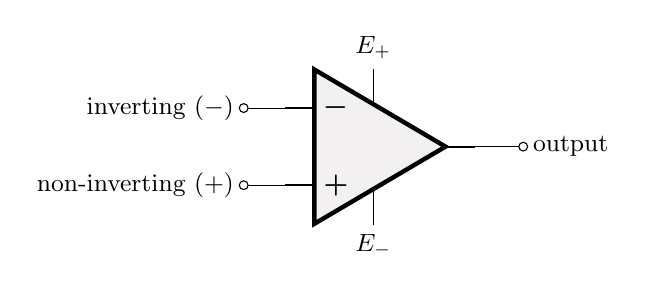
\begin{tikzpicture}[scale=0.9]
  \oaDevice
\end{tikzpicture}
\end{minipage}\hfill
\begin{minipage}[c]{0.46\linewidth}
The op-amp has (at least) five terminals: two inputs, one output and two supply terminals.
The supply terminals are connected to DC voltage sources $E_+ > E_-$. These values limit the
output voltage:
\[
  E_- \leq \vo \leq E_+ .
\]
\end{minipage}

All voltages are measured with respect to a common ground: $\vp$ at the non-inverting input,
$\vm$ at the inverting input and $\vo$ at the output. The supplies are usually symmetric,
$E_+ = \Es$ and $E_- = -\Es$, and they are often left out of the drawings.

\subsection{The transfer characteristic}

\begin{minipage}[c]{0.5\linewidth}
\centering
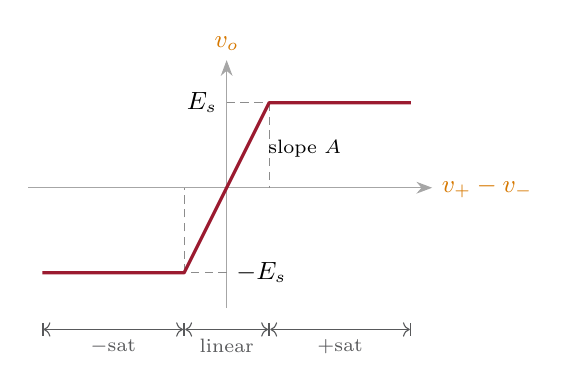
\begin{tikzpicture}[scale=0.9]
  \oaChar{1}
\end{tikzpicture}
\end{minipage}\hfill
\begin{minipage}[c]{0.46\linewidth}
The output depends on the difference $\Vcol{v_+ - v_-}$. Near zero the curve is a line with
slope $A$, the \textbf{open-loop voltage gain}. Typically $A \approx 2 \times 10^5$; this is why op-amps are also called \textbf{high-gain amplifiers}. Further
away the output is stuck at a supply value: the op-amp \textbf{saturates}.
\end{minipage}

The op-amp has three operating regions:
\begin{center}
\renewcommand{\arraystretch}{1.3}
\begin{tabular}{@{}lll@{}}
\toprule
region & output & condition\\
\midrule
linear & $\vo = A\,(\Vcol{v_+ - v_-})$ & $-\Es \leq \vo \leq \Es$\\
positive saturation ($+$sat) & $\vo = \Es$ & $A\,(\Vcol{v_+ - v_-}) > \Es$\\
negative saturation ($-$sat) & $\vo = -\Es$ & $A\,(\Vcol{v_+ - v_-}) < -\Es$\\
\bottomrule
\end{tabular}
\end{center}
The linear region is very narrow. With $A = 2 \times 10^5$ and $\Es = 12\V$ it is
$|\Vcol{v_+ - v_-}| \leq 12 / (2 \times 10^5)\V = 60\,\mu\mathrm{V}$.
Used alone (\textbf{open loop}), with the inputs set by outside sources, the op-amp is almost
always saturated. It is useless as a linear amplifier this way. The next sections show how
feedback changes this.

%==============================================================
\section{Models of the op-amp}

\subsection{The dependent-source model}

\begin{minipage}[c]{0.5\linewidth}
\centering
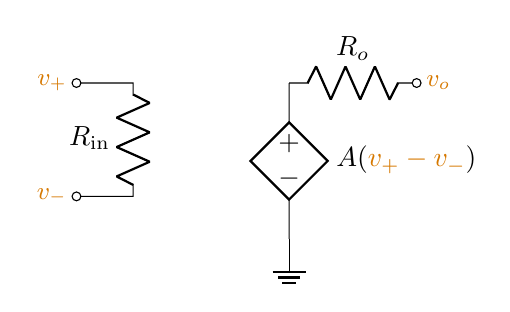
\begin{tikzpicture}[scale=0.9]
  \oaModel
\end{tikzpicture}
\end{minipage}\hfill
\begin{minipage}[c]{0.46\linewidth}
In the linear region the op-amp behaves like this circuit: an input resistance $R_{\mathrm{in}}$
between the inputs, and a voltage-controlled voltage source with an output resistance
$R_o$.
\end{minipage}

\begin{center}
\renewcommand{\arraystretch}{1.25}
\begin{tabular}{@{}lll@{}}
\toprule
parameter & meaning & typical value\\
\midrule
$R_{\mathrm{in}}$ & input resistance & $10^6$ -- $10^{12}\ohm$\\
$R_o$ & output resistance & $10$ -- $100\ohm$\\
$A$ & open-loop voltage gain & $10^5$ -- $10^8$\\
\bottomrule
\end{tabular}
\end{center}

\subsection{The finite-gain ideal model}

\begin{minipage}[c]{0.42\linewidth}
\centering
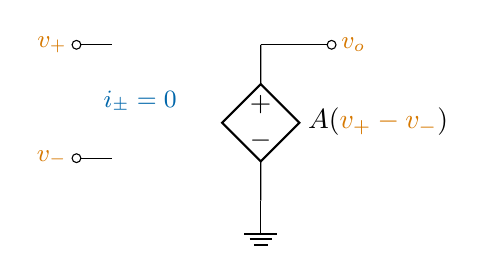
\begin{tikzpicture}[scale=0.9]
  \oaFGModel
\end{tikzpicture}
\end{minipage}\hfill
\begin{minipage}[c]{0.54\linewidth}
$R_{\mathrm{in}}$ is very large and $R_o$ is very small. Setting $R_{\mathrm{in}} = \infty$
and $R_o = 0$ gives the \textbf{finite-gain ideal model}. The gain $A$ is still finite, so
nothing unusual happens yet.
\end{minipage}
\[
  \ip = \im = 0, \qquad \vo = A\,(\vp - \vm) \quad\text{(linear region)} .
\]

%==============================================================
\needspace{12\baselineskip}
\section{Feedback}

\subsection{The follower with finite gain}

\begin{minipage}[c]{0.42\linewidth}
\centering
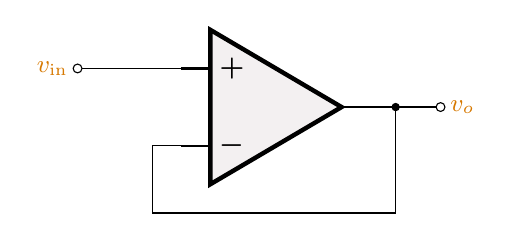
\begin{tikzpicture}[scale=0.95]
  \follower{0}
\end{tikzpicture}
\end{minipage}\hfill
\begin{minipage}[c]{0.54\linewidth}
Connect the output back to the inverting input. This is \textbf{negative feedback}. Now the
inputs are no longer set from outside: $\vm$ \emph{is} the output.
\[
  \vp = \vin, \qquad \vm = \vo .
\]
\end{minipage}

In the linear region, the finite-gain model gives
\[
  \vo = A\,(\vin - \vo)
  \quad\Rightarrow\quad
  \vo = \frac{A}{1 + A}\,\vin ,
  \qquad
  \vp - \vm = \vin - \vo = \frac{\vo}{A} .
\]
Take $\vin = 1\V$:
\begin{center}
\renewcommand{\arraystretch}{1.3}
\begin{tabular}{@{}lll@{}}
\toprule
$A$ & $\vo$ & $\vp - \vm$\\
\midrule
$10^5$ & $0.99999\V$ & $10\,\mu\mathrm{V}$\\
$10^6$ & $0.999999\V$ & $1\,\mu\mathrm{V}$\\
$10^8$ & $0.99999999\V$ & $0.01\,\mu\mathrm{V}$\\
\bottomrule
\end{tabular}
\end{center}
Two facts stand out.
\begin{itemize}
  \item The output is $\vo \approx \vin$ as long as $A$ is large. The circuit, not the op-amp, sets the
        gain.
  \item The input difference is tiny: the op-amp stays in its narrow linear region by itself.
\end{itemize}

\subsection{Why the difference stays small}

Redraw the follower as a feedback diagram, as in signals and control courses. The op-amp is a
block with gain $A$. Its input is the \emph{difference} $\Vcol{v_d} = \vp - \vm$. The input
$\vin$ enters with a $+$ sign; the output returns through the feedback path with a $-$ sign.

\begin{minipage}[c]{0.36\linewidth}
\centering
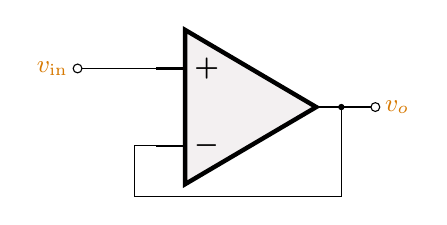
\begin{tikzpicture}[scale=0.72]
  \follower{0}
\end{tikzpicture}
\end{minipage}\hfill
\begin{minipage}[c]{0.62\linewidth}
\centering
\fbBlock{1}
\end{minipage}

\medskip
Follow the signal around the loop (the numbers are marked on the diagram):
\begin{enumerate}[label=\protect\cnum{\arabic*}, itemsep=2pt, leftmargin=*]
  \item Suppose $\vo$ is a little too high.
  \item The feedback path carries it back: $\vm = \vo$ rises too.
  \item $\vp = \vin$ is fixed, so the difference $\Vcol{v_d} = \vp - \vm$ falls.
  \item The block $A$ amplifies this: $\vo$ goes down.
\end{enumerate}
If $\vo$ is too low, every arrow reverses and $\vo$ goes up. Either way the loop corrects the
output. Reading the diagram,
\[
  \Vcol{v_d} = \vin - \vo, \qquad \vo = A\,\Vcol{v_d}
  \quad\Rightarrow\quad
  \Vcol{v_d} = \frac{\vin}{1 + A}, \qquad \vo = \frac{A}{1 + A}\,\vin .
\]
The difference is $\Vcol{v_d} = \vo / A$, at most $\Es / A$ (a few $\mu\mathrm{V}$). Negative
feedback adjusts the output until the two inputs are almost equal. Without feedback (open loop)
the lower path is missing: $\Vcol{v_d}$ is fixed from outside, nothing corrects the output, and
the op-amp saturates.

%==============================================================
\section{The infinite-gain ideal model}

Since the answers hardly depend on $A$ once it is large, let $A \to \infty$ in the follower
results:
\[
  \vo = \frac{A}{1 + A}\,\vin \;\to\; \vin, \qquad
  \Vcol{v_d} = \vp - \vm = \frac{\vin}{1 + A} \;\to\; 0 .
\]
\begin{itemize}
  \item The output follows the input exactly: the circuit sets the gain, not $A$.
  \item An infinite gain with a finite output is possible only if its input is zero. The
        feedback loop drives $\vp - \vm$ to $0$. This is the linear region, $\vp = \vm$.
  \item If $|\vin| > \Es$, the output cannot follow. The loop can no longer make $\Vcol{v_d}$
        zero, and the op-amp saturates on the side given by the sign of $\Vcol{v_d} = \vp - \vm$.
\end{itemize}
These three cases give the \textbf{infinite-gain ideal model}.

\begin{minipage}[c]{0.44\linewidth}
\centering
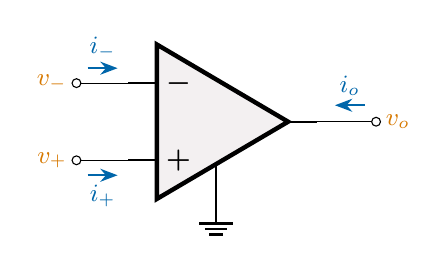
\begin{tikzpicture}[scale=0.95]
  \oaVolt
\end{tikzpicture}
\end{minipage}\hfill
\begin{minipage}[c]{0.52\linewidth}
\centering
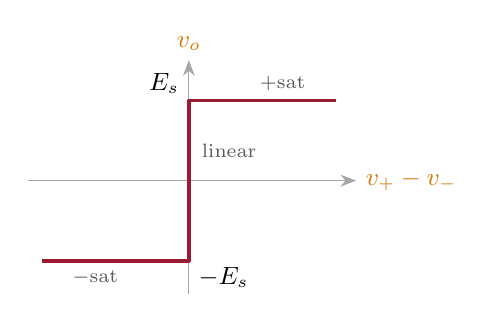
\begin{tikzpicture}[scale=0.85]
  \oaIdealChar
\end{tikzpicture}
\end{minipage}

\begin{definitionbox}{The infinite-gain ideal op-amp}
In \textbf{every} region the input currents are zero: $\ip = \im = 0$. The three regions are
\begin{center}
\renewcommand{\arraystretch}{1.3}
\begin{tabular}{@{}lll@{}}
\toprule
linear & $+$sat & $-$sat\\
\midrule
$\vp = \vm$ & $\vp > \vm$ & $\vp < \vm$\\
$-\Es \leq \vo \leq \Es$ & $\vo = \Es$ & $\vo = -\Es$\\
\bottomrule
\end{tabular}
\end{center}
\end{definitionbox}

Read the linear row correctly:
\begin{itemize}
  \item $\vp = \vm$ is not a property of the op-amp alone. It is what the feedback produces when
        the op-amp works in the linear region.
  \item $\vp = \vm$ does \textbf{not} mean the inputs are connected. No current flows between
        them.
  \item The output current $\Icol{i_o}$ is \textbf{not} zero. The output can deliver current;
        the power comes from the supplies. So do not write KCL at the output node: $\Icol{i_o}$ is
        unknown there.
\end{itemize}

%==============================================================
\section{Analysing an op-amp circuit}

The method is the one used for the ideal diode: assume a region, use the equation of that
region, then check the condition of that region. For the diode it was ``ON: $v = 0$, check
$i \geq 0$''. For the ideal op-amp there are three regions:

\begin{center}
\renewcommand{\arraystretch}{1.35}
\begin{tabular}{@{}lll@{}}
\toprule
region & assume (use this equation) & check (this must hold)\\
\midrule
linear & $\vp = \vm$ & $-\Es \leq \vo \leq \Es$\\
$+$sat & $\vo = \Es$ & $\vp > \vm$\\
$-$sat & $\vo = -\Es$ & $\vp < \vm$\\
\bottomrule
\end{tabular}
\end{center}
In all three regions $\ip = \im = 0$, so KCL at the input nodes can be written before choosing a
region. We do not know in advance which region an input puts the op-amp in. So we try all three,
and each region holds for the inputs that pass its check. Together the three pieces give the
transfer characteristic.

\begin{ideabox}[Analysing an op-amp circuit]
\begin{enumerate}[itemsep=2pt]
  \item \textbf{Every region:} KCL at the input nodes ($\ip = \im = 0$) gives $\vp$ and $\vm$ in
        terms of the inputs and $\vo$.
  \item \textbf{Linear:} set $\vp = \vm$, solve for $\vo$, keep the inputs with $|\vo| \leq \Es$.
  \item \textbf{$+$sat:} set $\vo = \Es$, keep the inputs with $\vp > \vm$.
  \item \textbf{$-$sat:} set $\vo = -\Es$, keep the inputs with $\vp < \vm$.
  \item \textbf{Join} the three pieces: the transfer characteristic.
\end{enumerate}
\end{ideabox}

\subsection{Step 1: KCL at the inputs}

The op-amp draws no current at its inputs ($\ip = \im = 0$). So at an input node only the
external elements carry current, and KCL there is an ordinary node equation: the op-amp does not
appear in it. Take the circuit below (the inverting amplifier, analysed later).

\begin{minipage}[c]{0.5\linewidth}
\centering
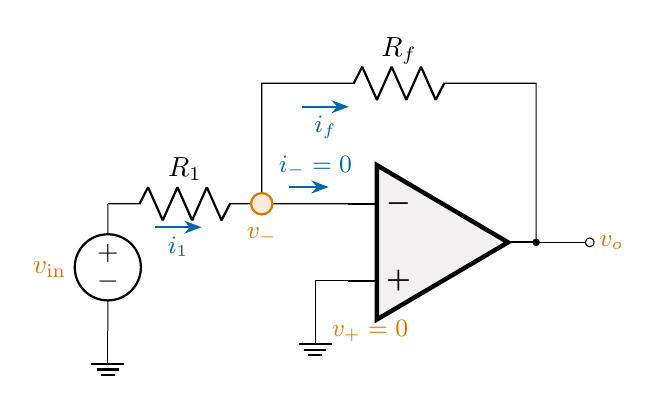
\begin{tikzpicture}[scale=0.85]
  \kclFig
\end{tikzpicture}
\end{minipage}\hfill
\begin{minipage}[c]{0.46\linewidth}
\textbf{$+$ input:} it is grounded, so $\vp = 0$.

\smallskip
\textbf{$-$ input:} KCL at node $\vm$,
\[
  \Icol{i_1} = \Icol{i_f} + \underbrace{\im}_{0}
  \;\Rightarrow\;
  \frac{\vin - \vm}{R_1} = \frac{\vm - \vo}{R_f} .
\]
\end{minipage}

\smallskip
Solving for $\vm$:
\[
  \vm = \frac{R_f\,\vin + R_1\,\vo}{R_1 + R_f} .
\]
\begin{itemize}
  \item These relations hold in \textbf{every} region, because $\ip = \im = 0$ in every region.
  \item $\vo$ is still unknown and stays as a symbol. Each region supplies the missing equation:
        $\vp = \vm$ (linear) or $\vo = \pm\Es$ (saturation).
  \item Do \textbf{not} write KCL at the output node. The op-amp output current $\Icol{i_o}$ is
        unknown, so that equation only adds a new unknown.
\end{itemize}
In the follower below, step 1 needs no KCL at all: the $+$ input is the input node and the $-$
input is wired to the output.



\subsection{The method on the voltage follower}

\begin{minipage}[c]{0.38\linewidth}
\centering
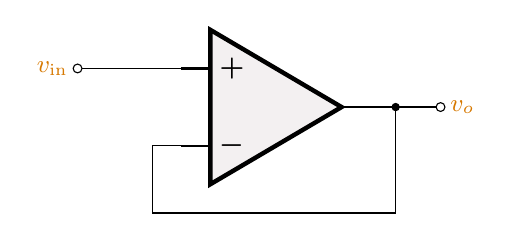
\begin{tikzpicture}[scale=0.95]
  \follower{0}
\end{tikzpicture}
\end{minipage}\hfill
\begin{minipage}[c]{0.58\linewidth}
Find $\vo$ as a function of $\vin$ with the infinite-gain model.
\end{minipage}

\solstep{1}{Every region}
No KCL is needed here: the $+$ input is the input node and the $-$ input is wired to the output:
\[
  \vp = \vin, \qquad \vm = \vo .
\]

\solstep{2}{Linear}
Assume $\vp = \vm$: \ $\vo = \vin$. \
Check $|\vo| \leq \Es$: \ $|\vin| \leq \Es$.

\solstep{3}{$+$sat}
Assume $\vo = \Es$, so $\vm = \Es$. \
Check $\vp > \vm$: \ $\vin > \Es$.

\solstep{4}{$-$sat}
Assume $\vo = -\Es$, so $\vm = -\Es$. \
Check $\vp < \vm$: \ $\vin < -\Es$.

\solstep{5}{Join}
\begin{minipage}[c]{0.5\linewidth}
The three ranges cover the whole $\vin$ axis without overlap, so every input has exactly one
solution. The output follows the input with gain 1, up to the supply limits.
\end{minipage}\hfill
\begin{minipage}[c]{0.46\linewidth}
\centering
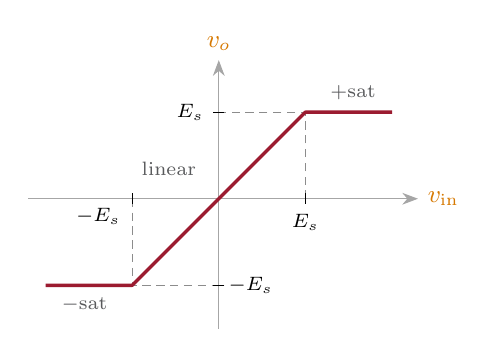
\begin{tikzpicture}[x=0.55cm, y=0.55cm]
  \tax{-4.4}{4.6}{-3.0}{3.2}{$\vin$}{$\vo$}
  \draw[gdash] (2,0) -- (2,2) -- (0,2); \draw[gdash] (-2,0) -- (-2,-2) -- (0,-2);
  \draw[crv] (-4,-2) -- (-2,-2) -- (2,2) -- (4,2);
  \xt{2}{$\Es$} \draw ([yshift=2pt]-2,0) -- ([yshift=-2pt]-2,0); \node[font=\scriptsize, anchor=north east] at (-2.05,0) {$-\Es$}; \yt{2}{$\Es$} \ytr{-2}{$-\Es$}
  \node[reg, below] at (-3.1,-2.05) {$-$sat};
  \node[reg, above] at (3.1,2.05) {$+$sat};
  \node[reg, anchor=south east] at (-0.3,0.3) {linear};
\end{tikzpicture}
\end{minipage}

%==============================================================
\section{The voltage follower in use}

\subsection{The follower as a buffer}

Why use a circuit with gain 1? Many voltage sources in practice are not ideal: a sensor, a
voltage divider or a potentiometer behaves like a source $\Vcol{v_s}$ with an internal
resistance $R_s$. Connect a load $R_L$ to it directly and the voltage drops to
$\Vcol{v_s}\,R_L/(R_s + R_L)$. Put a follower in between:

\begin{minipage}[c]{0.6\linewidth}
\centering
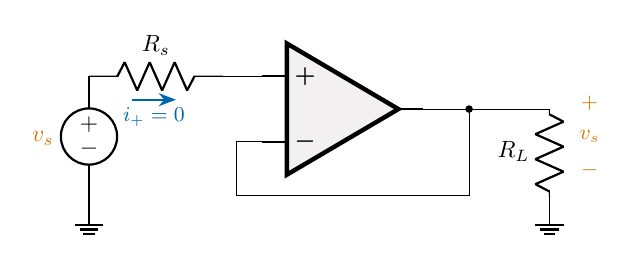
\begin{tikzpicture}[scale=0.85, transform shape]
  \bufThev
\end{tikzpicture}
\end{minipage}\hfill
$\Longrightarrow$\hfill
\begin{minipage}[c]{0.3\linewidth}
\centering
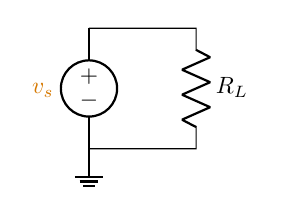
\begin{tikzpicture}[scale=0.85, transform shape]
  \bufEquiv
\end{tikzpicture}
\end{minipage}

\begin{itemize}
  \item \textbf{Input side.} $\ip = 0$, so no current flows in $R_s$ and there is no drop on
        it: $\vp = \Vcol{v_s}$ exactly, whatever $R_s$ is.
  \item \textbf{Output side.} $\vo = \vp = \Vcol{v_s}$, whatever $R_L$ is. The op-amp output
        behaves like an ideal voltage source; the load current comes from the supplies, not
        from the source.
  \item \textbf{Result.} The load sees $\Vcol{v_s}$ as if an ideal source were connected to it
        (right). The source and the load are isolated from each other. The voltage gain is 1,
        but the power delivered to the load comes from the supplies.
\end{itemize}
Typical uses: reading a sensor with a high internal resistance; taking a reference voltage
from a divider or a potentiometer and driving a load with it; separating two stages, so that
connecting the second one does not change the first. The limits are those of the op-amp:
$|\vo| \leq \Es$ and a maximum output current (typically a few tens of mA).

\bigskip
\begin{examplebox}[Example 16.1 --- loading and buffering]
\begin{center}
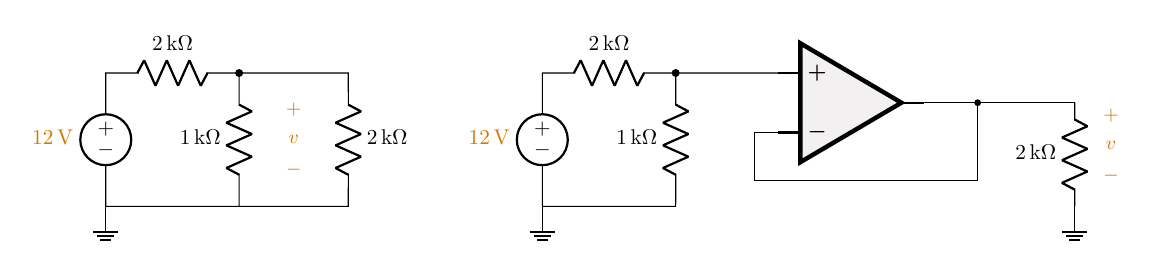
\begin{tikzpicture}[scale=0.77, transform shape]
  \bufEx{0}
  \begin{scope}[xshift=7.2cm] \bufEx{1} \end{scope}
\end{tikzpicture}
\end{center}
A divider gives $4\V$ when nothing is connected to it. Find $\Vcol{v}$ on a $2\kohm$ load
connected directly (left) and through a voltage follower (right).
\end{examplebox}

\solution

\solstep{1}{Direct connection}
The $1\kohm$ and the $2\kohm$ load are in parallel: $1 \parallel 2 = \tfrac23\kohm$. The divider gives
\[
  \Vcol{v} = 12 \cdot \frac{2/3}{2 + 2/3} = 12 \cdot \frac{2/3}{8/3} = 3\V .
\]
The load pulls the voltage down from $4\V$ to $3\V$.

\solstep{2}{Through the follower}
$\ip = 0$, so the divider is unloaded and $\vp = 4\V$. In the linear region $\vo = \vp$, so
\[
  \Vcol{v} = 4\V ,
\]
whatever the load is. The load current $4\V / 2\kohm = 2\mA$ comes from the op-amp output, not
from the divider.

\subsection{Positive feedback}

\begin{minipage}[c]{0.42\linewidth}
\centering
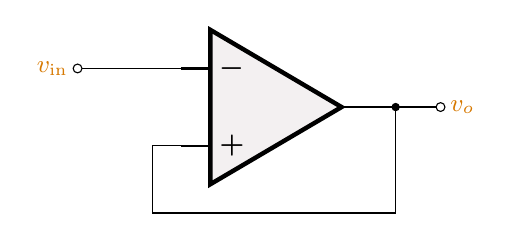
\begin{tikzpicture}[scale=0.95]
  \follower{1}
\end{tikzpicture}
\end{minipage}\hfill
\begin{minipage}[c]{0.54\linewidth}
Swap the two inputs. The output now goes back to the \emph{non-inverting} input:
\[
  \vm = \vin, \qquad \vp = \vo .
\]
This is \textbf{positive feedback}.
\end{minipage}

\paragraph{The loop.} Draw the feedback diagram as for the follower. The only change is the
sign at the difference: the fed-back signal $\vp = \vo$ now enters with a $+$ sign, and $\vin$
with a $-$ sign.

\begin{minipage}[c]{0.5\linewidth}
\centering
\fbBlockPos{1}
\end{minipage}\hfill
\begin{minipage}[c]{0.46\linewidth}
\begin{enumerate}[label=\protect\cnum{\arabic*}, itemsep=2pt, leftmargin=*]
  \item Suppose $\vo$ is a little too high.
  \item The feedback path carries it back: $\vp = \vo$ rises.
  \item $\vm = \vin$ is fixed, so $\Vcol{v_d} = \vp - \vm$ \emph{rises}.
  \item The op-amp amplifies this: $\vo$ goes \emph{further up}.
\end{enumerate}
\end{minipage}

\smallskip
With negative feedback, step 3 was ``$\Vcol{v_d}$ falls'' and the loop pulled $\vo$ back. Here
every pass around the loop makes the deviation larger, until $\vo$ reaches $\Es$ (or $-\Es$ if
the first deviation was downwards).

\paragraph{The equations still have a linear solution.} With finite gain,
\[
  \vo = A\,(\vp - \vm) = A\,(\vo - \vin)
  \quad\Rightarrow\quad
  \vo = \frac{A}{A - 1}\,\vin \approx \vin ,
\]
the same answer as the follower. But the circuit does not stay there: the smallest disturbance
grows around the loop. A solution of the equations is not enough; it must also be
\textbf{stable}. Our models have no time behaviour, so they cannot show this directly; the full
treatment needs dynamic models (later courses).

\needspace{12\baselineskip}
\textbf{Step 1: the three regions.} With the ideal model, $\vm = \vin$ and $\vp = \vo$. In
saturation $\vo$ is known, so $\vp$ is known too; the check compares it with $\vm = \vin$:\par\smallskip

\begin{center}
\renewcommand{\arraystretch}{1.3}
\begin{tabular}{@{}lll@{}}
\toprule
region & assume & check $\Rightarrow$ valid for\\
\midrule
linear & $\vo = \vin$ & $|\vo| \leq \Es \Rightarrow |\vin| \leq \Es$\\
$+$sat & $\vo = \Es$ & $\underbrace{\Es}_{\vp} > \underbrace{\vin}_{\vm} \Rightarrow \vin < \Es$\\
$-$sat & $\vo = -\Es$ & $\underbrace{-\Es}_{\vp} < \underbrace{\vin}_{\vm} \Rightarrow \vin > -\Es$\\
\bottomrule
\end{tabular}
\end{center}

\begin{minipage}[c]{0.5\linewidth}
Draw each piece only over its valid range. Unlike the follower, the ranges \emph{overlap}: for
$-\Es < \vin < \Es$ all three pieces are present.
\end{minipage}\hfill
\begin{minipage}[c]{0.46\linewidth}
\centering
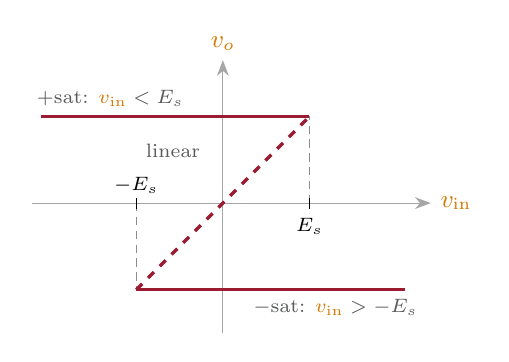
\begin{tikzpicture}[x=0.55cm, y=0.55cm]
  \pfPlot{0}
\end{tikzpicture}
\end{minipage}

\textbf{Step 2: drop the unstable piece.} The linear piece (dashed) is unstable, as the loop
showed. Only the two saturated pieces remain.

\needspace{8\baselineskip}
\textbf{Step 3: follow the output as $\vin$ changes slowly.}
\begin{itemize}\itemsep2pt
  \item \textcolor{swup}{\textbf{Increasing $\vin$}} (solid arrows). Start with $\vin < -\Es$:
        only $+$sat is valid, so $\vo = \Es$. As $\vin$ increases, $+$sat stays valid while
        $\vin < \Es$, so $\vo$ stays at $\Es$, even after $-$sat also becomes possible.
  \item At $\vin = \Es$ the $+$sat condition $\vp = \Es > \vm = \vin$ fails. The only valid
        stable piece left is $-$sat: $\vo$ \textbf{jumps} to $-\Es$.
  \item \textcolor{swdn}{\textbf{Decreasing $\vin$}} (dashed arrows). By the same argument $\vo$
        stays at $-\Es$ until $\vin = -\Es$, then jumps to $+\Es$.
\end{itemize}
\begin{center}
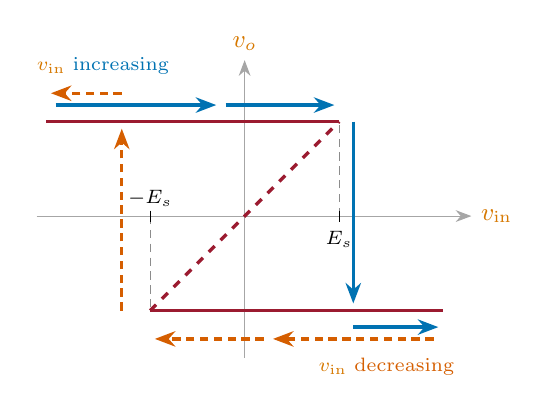
\begin{tikzpicture}[x=0.6cm, y=0.6cm]
  \pfPlot{1}
\end{tikzpicture}
\end{center}
For $-\Es < \vin < \Es$ the output depends on where it came from: the circuit \emph{remembers}
its past. The two paths form a loop; this behaviour is called \textbf{hysteresis}. The circuit
does not follow the input; it \emph{switches} between $+\Es$ and $-\Es$.

\paragraph{Conclusion.} For an amplifier the feedback must go to the \textbf{inverting} input. In
design and in the laboratory we do not connect the output to the non-inverting input when we want
linear operation.

Positive feedback is not useless, though. Some circuits use it on purpose: circuits whose output
jumps between two values (switching circuits), and circuits that produce a signal by themselves
(oscillators). These are not amplifiers; you will meet them in later courses.

%==============================================================
\section{Inverting and non-inverting amplifiers}

\subsection{The inverting amplifier}

\begin{minipage}[c]{0.46\linewidth}
\centering
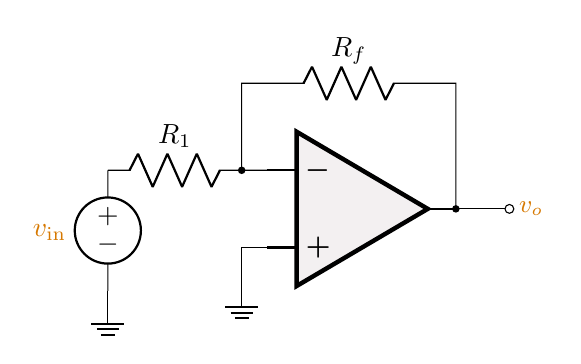
\begin{tikzpicture}[scale=0.85]
  \invAmp{$R_1$}{$R_f$}{$\Vcol{v_{\mathrm{in}}}$}
\end{tikzpicture}
\end{minipage}\hfill
\begin{minipage}[c]{0.5\linewidth}
\textbf{In every region.} $\vp = 0$. KCL at the inverting input, with $\im = 0$:
\[
  \frac{\vm - \vin}{R_1} + \frac{\vm - \vo}{R_f} = 0 ,
\]
\[
  \vm = \frac{R_f\,\vin + R_1\,\vo}{R_1 + R_f} .
\]
\end{minipage}

\textbf{Linear.} $\vm = \vp = 0$ gives $R_f\,\vin + R_1\,\vo = 0$:
\[
  \vo = -\frac{R_f}{R_1}\,\vin , \qquad \text{valid for } -\frac{R_1}{R_f}\Es \leq \vin \leq \frac{R_1}{R_f}\Es .
\]
\textbf{$+$sat.} $\vo = \Es$ and $\vm < \vp = 0$: $R_f\,\vin + R_1\Es < 0$, so $\vin < -\frac{R_1}{R_f}\Es$.

\textbf{$-$sat.} $\vo = -\Es$ and $\vm > 0$: $\vin > \frac{R_1}{R_f}\Es$.

The gain is $-R_f/R_1$: it depends only on two resistors, not on the op-amp. The inverting
input stays at $0\V$ although it is not connected to ground; it is called a \textbf{virtual
ground}. So the input current is $\vin/R_1$, and the source sees an input resistance $R_1$.

\bigskip
\begin{examplebox}[Example 16.2 --- an inverting amplifier]
\begin{minipage}[c]{0.46\linewidth}
\centering
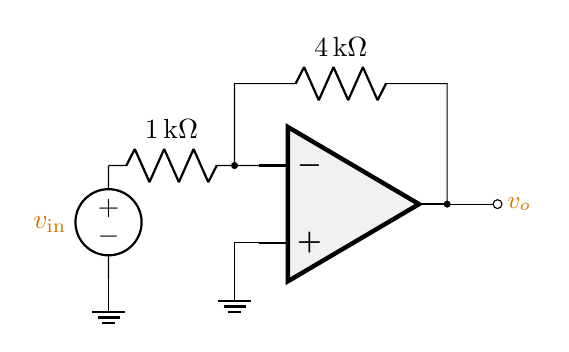
\begin{tikzpicture}[scale=0.8]
  \invAmp{$1\kohm$}{$4\kohm$}{$\Vcol{v_{\mathrm{in}}}$}
\end{tikzpicture}
\end{minipage}\hfill
\begin{minipage}[c]{0.5\linewidth}
The supplies are $\pm 12\V$. Draw the transfer characteristic. Find $\vo$ for
$\vin = 2\V$ and for $\vin = 5\V$.
\end{minipage}
\end{examplebox}

\solution

\solstep{1}{The three regions}
\begin{minipage}[c]{0.52\linewidth}
Gain: $-R_f/R_1 = -4$. Linear: $\vo = -4\,\vin$ for $|\vin| \leq \frac14 \cdot 12 = 3\V$.
$+$sat for $\vin < -3\V$; $-$sat for $\vin > 3\V$.
\end{minipage}\hfill
\begin{minipage}[c]{0.44\linewidth}
\centering
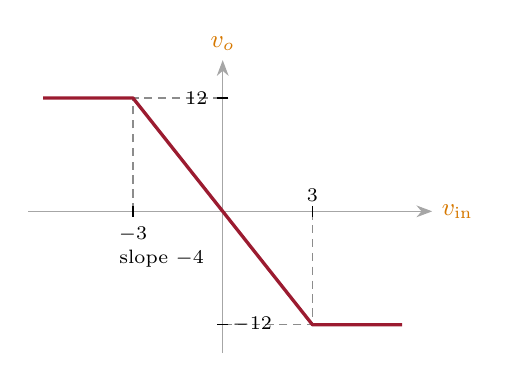
\begin{tikzpicture}[x=0.38cm, y=0.12cm]
  \tax{-6.5}{7}{-15}{16}{$\vin$}{$\vo$}
  \draw[gdash] (3,0) -- (3,-12) -- (0,-12); \draw[gdash] (-3,0) -- (-3,12) -- (0,12);
  \draw[crv] (-6,12) -- (-3,12) -- (3,-12) -- (6,-12);
  \xtu{3}{$3$} \xt{-3}{$-3$} \yt{12}{$12$} \ytr{-12}{$-12$}
  \node[font=\scriptsize, anchor=east] at (-0.3,-5) {slope $-4$};
\end{tikzpicture}
\end{minipage}

\solstep{2}{The two inputs}
$\vin = 2\V$ is in the linear range: $\vo = -8\V$. $\vin = 5\V$ is beyond $3\V$: the op-amp is in
$-$sat and $\vo = -12\V$, not $-20\V$.

\subsection{The non-inverting amplifier}

\begin{minipage}[c]{0.46\linewidth}
\centering
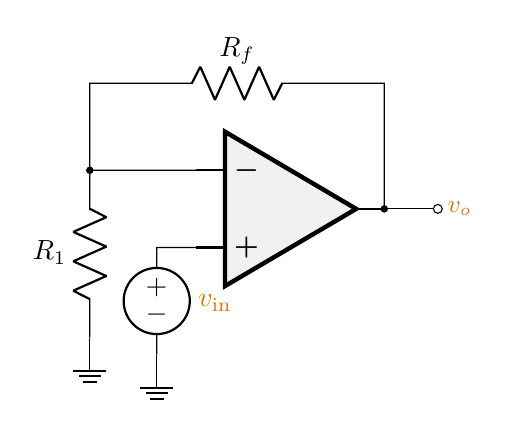
\begin{tikzpicture}[scale=0.85]
  \noninvAmp{$R_1$}{$R_f$}{$\Vcol{v_{\mathrm{in}}}$}
\end{tikzpicture}
\end{minipage}\hfill
\begin{minipage}[c]{0.5\linewidth}
\textbf{In every region.} $\vp = \vin$. KCL at the inverting input ($\im = 0$): $R_1$ and $R_f$
form a divider,
\[
  \vm = \frac{R_1}{R_1 + R_f}\,\vo .
\]
\end{minipage}

\textbf{Linear.} $\vm = \vp$:
\[
  \vo = \Big(1 + \frac{R_f}{R_1}\Big)\vin , \qquad \text{valid for }
  |\vin| \leq \frac{\Es}{1 + R_f/R_1} .
\]
\textbf{$+$sat.} $\vo = \Es$, $\vp > \vm$: $\vin > \Es/(1 + R_f/R_1)$. \quad
\textbf{$-$sat.} $\vin < -\Es/(1 + R_f/R_1)$.

The gain $1 + R_f/R_1$ is positive and at least 1. The source sees an open circuit
($\ip = 0$). The voltage follower is the special case $R_f = 0$, $R_1 = \infty$.

\bigskip
\begin{examplebox}[Example 16.3 --- a non-inverting amplifier]
With $R_1 = 1\kohm$, $R_f = 3\kohm$ and supplies $\pm 12\V$, draw the transfer characteristic.
Find $\vo$ for $\vin = 1.5\V$ and for $\vin = -4\V$.
\end{examplebox}

\solution

\solstep{1}{The three regions}
\begin{minipage}[c]{0.52\linewidth}
Gain: $1 + 3 = 4$. Linear: $\vo = 4\,\vin$ for $|\vin| \leq 12/4 = 3\V$. $+$sat for
$\vin > 3\V$; $-$sat for $\vin < -3\V$.
\end{minipage}\hfill
\begin{minipage}[c]{0.44\linewidth}
\centering
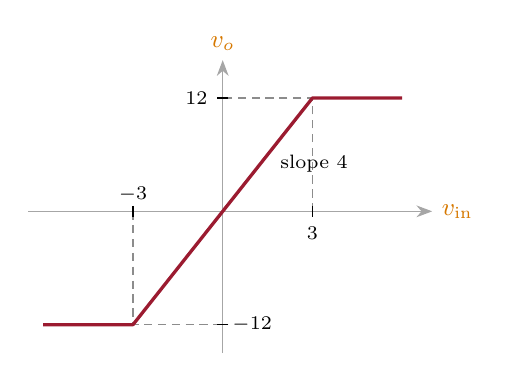
\begin{tikzpicture}[x=0.38cm, y=0.12cm]
  \tax{-6.5}{7}{-15}{16}{$\vin$}{$\vo$}
  \draw[gdash] (3,0) -- (3,12) -- (0,12); \draw[gdash] (-3,0) -- (-3,-12) -- (0,-12);
  \draw[crv] (-6,-12) -- (-3,-12) -- (3,12) -- (6,12);
  \xt{3}{$3$} \xtu{-3}{$-3$} \yt{12}{$12$} \ytr{-12}{$-12$}
  \node[font=\scriptsize, anchor=west] at (1.6,5) {slope $4$};
\end{tikzpicture}
\end{minipage}

\solstep{2}{The two inputs}
$\vin = 1.5\V$: linear, $\vo = 6\V$. $\vin = -4\V$: $-$sat, $\vo = -12\V$.

%==============================================================
\section{Summing and difference amplifiers}

From here on we assume the linear region and check $-\Es \leq \vo \leq \Es$ at the end.

\subsection{The summing amplifier}

\begin{minipage}[c]{0.46\linewidth}
\centering
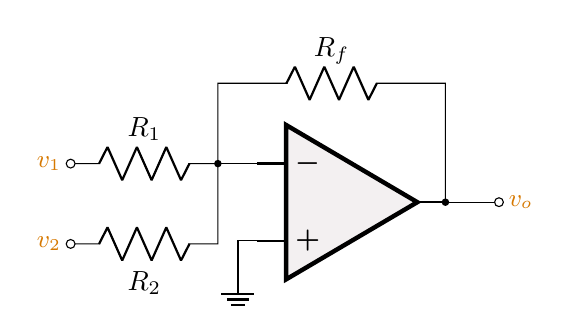
\begin{tikzpicture}[scale=0.85]
  \summing{$R_1$}{$R_2$}{$R_f$}
\end{tikzpicture}
\end{minipage}\hfill
\begin{minipage}[c]{0.5\linewidth}
The inverting input is a virtual ground: $\vm = \vp = 0$. Each input sends the current
$\Vcol{v_k}/R_k$ into the node, and all of it flows through $R_f$ ($\im = 0$):
\[
  \frac{\Vcol{v_1}}{R_1} + \frac{\Vcol{v_2}}{R_2} = -\frac{\vo}{R_f} .
\]
\end{minipage}

\[
  \vo = -\Big(\frac{R_f}{R_1}\,\Vcol{v_1} + \frac{R_f}{R_2}\,\Vcol{v_2}\Big) .
\]
With $n$ inputs: $\vo = -\sum_k (R_f/R_k)\,\Vcol{v_k}$. The inputs do not affect each other,
because the node they meet at is held at $0\V$.

\bigskip
\begin{examplebox}[Example 16.4 --- design an adder]
Design a circuit with $\vo = -(2\,\Vcol{v_1} + \Vcol{v_2})$. Check it with $\Vcol{v_1} = 1\V$ and
$\Vcol{v_2} = 2\V$.
\end{examplebox}

\solution

\solstep{1}{Choose the resistors}
Take $R_f = 2\kohm$. Then $R_f/R_1 = 2$ gives $R_1 = 1\kohm$, and $R_f/R_2 = 1$ gives
$R_2 = 2\kohm$.

\solstep{2}{Check}
$\vo = -(2 \cdot 1 + 2) = -4\V$, inside $\pm 12\V$. \ \yes

\subsection{The difference amplifier}

\begin{minipage}[c]{0.46\linewidth}
\centering
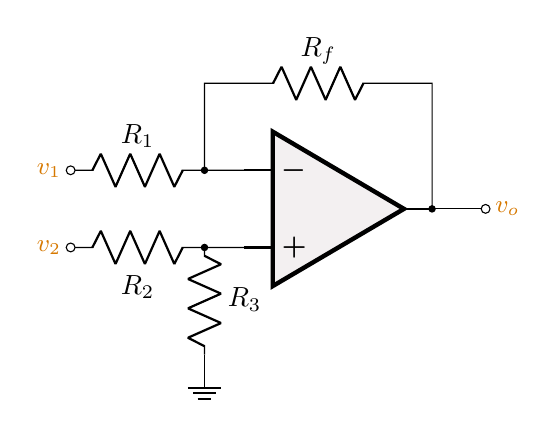
\begin{tikzpicture}[scale=0.85]
  \difference{$R_1$}{$R_2$}{$R_3$}{$R_f$}
\end{tikzpicture}
\end{minipage}\hfill
\begin{minipage}[c]{0.5\linewidth}
\textbf{Non-inverting input.} A divider ($\ip = 0$):
\[
  \vp = \frac{R_3}{R_2 + R_3}\,\Vcol{v_2} .
\]
\textbf{Inverting input.} KCL as in the inverting amplifier:
\[
  \vm = \frac{R_f\,\Vcol{v_1} + R_1\,\vo}{R_1 + R_f} .
\]
\end{minipage}

\textbf{Linear.} $\vm = \vp$ gives
\[
  \vo = \Big(1 + \frac{R_f}{R_1}\Big)\frac{R_3}{R_2 + R_3}\,\Vcol{v_2} - \frac{R_f}{R_1}\,\Vcol{v_1} .
\]
Choose the resistors with $\dfrac{R_f}{R_1} = \dfrac{R_3}{R_2}$. Then the first coefficient is also
$R_f/R_1$, and
\[
  \vo = \frac{R_f}{R_1}\,(\Vcol{v_2} - \Vcol{v_1}) .
\]
The output depends only on the difference of the inputs.

\bigskip
\begin{examplebox}[Example 16.5 --- a difference amplifier]
Take $R_1 = R_2 = 1\kohm$ and $R_f = R_3 = 3\kohm$. Find $\vo$ for $\Vcol{v_1} = 2\V$,
$\Vcol{v_2} = 3\V$, and for $\Vcol{v_1} = \Vcol{v_2} = 5\V$.
\end{examplebox}

\solution

\solstep{1}{The gain}
$R_f/R_1 = 3 = R_3/R_2$, so $\vo = 3\,(\Vcol{v_2} - \Vcol{v_1})$.

\solstep{2}{The two inputs}
$\vo = 3\,(3 - 2) = 3\V$. With equal inputs, $\vo = 0$: a voltage common to both inputs is
rejected.

%==============================================================
\section{Integrator and differentiator}

A capacitor $C$ relates its current and voltage by $\Icol{i} = C\,d\Vcol{v_C}/dt$, or
\[
  \Vcol{v_C}(t) = \Vcol{v_C}(0) + \frac{1}{C}\int_0^t \Icol{i}(\tau)\,d\tau .
\]
(Capacitors are treated in detail in later lectures.) Put a capacitor in place of a resistor in
the inverting amplifier.

\subsection{The integrator}

\begin{minipage}[c]{0.46\linewidth}
\centering
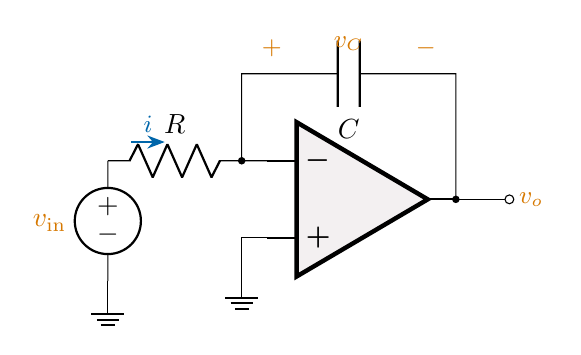
\begin{tikzpicture}[scale=0.85]
  \intdiff{0}
\end{tikzpicture}
\end{minipage}\hfill
\begin{minipage}[c]{0.5\linewidth}
Linear region: $\vm = 0$. Then
\[
  \Icol{i} = \frac{\vin}{R}, \qquad \Vcol{v_C} = \vm - \vo = -\vo .
\]
The current $\Icol{i}$ flows on into the capacitor ($\im = 0$).
\end{minipage}

Put both into the capacitor equation:
\[
  \vo(t) = \vo(0) - \frac{1}{RC}\int_0^t \vin(\tau)\,d\tau .
\]

\bigskip
\begin{examplebox}[Example 16.6 --- an integrator saturates]
An integrator has $R = 1\kohm$, $C = 1\mF$ ($RC = 1\s$) and supplies $\pm 12\V$, with
$\vo(0) = 0$. At $t = 0$ the input jumps to $\vin = 2\V$ and stays there. Find $\vo(t)$.
\end{examplebox}

\solution

\solstep{1}{Linear region}
\begin{minipage}[c]{0.52\linewidth}
\[
  \vo(t) = -\frac{1}{1}\int_0^t 2\,d\tau = -2t \ \mathrm{V}.
\]
The output falls along a ramp.
\end{minipage}\hfill
\begin{minipage}[c]{0.44\linewidth}
\centering
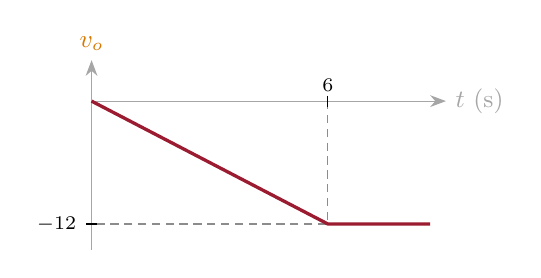
\begin{tikzpicture}[x=0.5cm, y=0.13cm]
  \draw[vax] (0,0) -- (9,0) node[right, font=\small] {$t$ (s)};
  \draw[vax] (0,-14.5) -- (0,4) node[above, font=\small] {$\vo$};
  \draw[gdash] (6,0) -- (6,-12) -- (0,-12);
  \draw[crv] (0,0) -- (6,-12) -- (8.6,-12);
  \xtu{6}{$6$} \yt{-12}{$-12$}
\end{tikzpicture}
\end{minipage}

\solstep{2}{Saturation}
The ramp reaches $-12\V$ at $t = 6\s$. After that the op-amp is in $-$sat and $\vo = -12\V$.

\subsection{The differentiator}

\begin{minipage}[c]{0.46\linewidth}
\centering
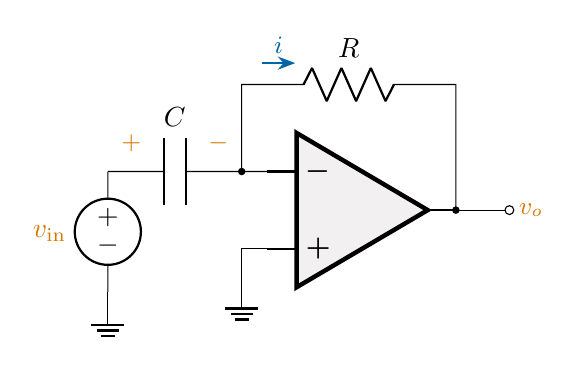
\begin{tikzpicture}[scale=0.85]
  \intdiff{1}
\end{tikzpicture}
\end{minipage}\hfill
\begin{minipage}[c]{0.5\linewidth}
Linear region: $\vm = 0$, so the capacitor voltage is $\vin$:
\[
  \Icol{i} = C\,\frac{d\vin}{dt}, \qquad \vo = -R\,\Icol{i} .
\]
\end{minipage}

\[
  \vo(t) = -RC\,\frac{d\vin}{dt} .
\]
For example, with $RC = 1\s$ and the ramp $\vin = 3t$ V, the output is the constant
$\vo = -3\V$.

%==============================================================
\section{Limits of the ideal model: finite gain}

Earlier we saw that the follower has gain $A/(1 + A)$, which is $0.99999$ for $A = 10^5$. One
more check, on the inverting amplifier, shows how small the error of the ideal model is.

\begin{examplebox}[Example 16.7 --- inverting amplifier with finite gain]
\begin{minipage}[c]{0.46\linewidth}
\centering
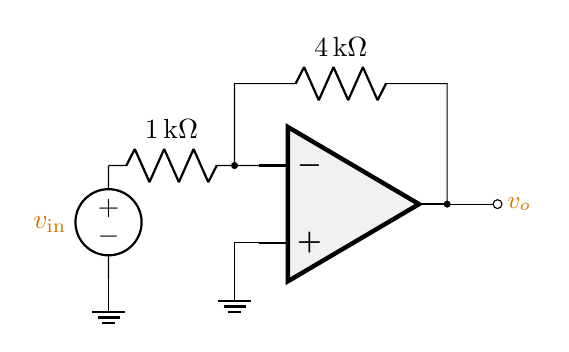
\begin{tikzpicture}[scale=0.8]
  \invAmp{$1\kohm$}{$4\kohm$}{$\Vcol{v_{\mathrm{in}}}$}
\end{tikzpicture}
\end{minipage}\hfill
\begin{minipage}[c]{0.5\linewidth}
Use the finite-gain model with $A = 10^5$ (linear region). Find the gain $\vo/\vin$ and compare
it with the ideal value $-4$.
\end{minipage}
\end{examplebox}

\solution

\solstep{1}{Equations}
$\vp = 0$, so the op-amp gives $\vo = A(0 - \vm) = -A\,\vm$. KCL at $\vm$ ($\im = 0$):
\[
  \frac{\vm - \vin}{1} + \frac{\vm - \vo}{4} = 0
  \quad\Rightarrow\quad
  \vm = \frac{4\,\vin + \vo}{5} .
\]

\solstep{2}{Gain}
Substitute $\vm = -\vo/A$:
\[
  -\frac{\vo}{A} = \frac{4\,\vin + \vo}{5}
  \quad\Rightarrow\quad
  \frac{\vo}{\vin} = -\frac{4}{1 + 5/A} = -\frac{4}{1.00005} = -3.9998 .
\]

\solstep{3}{Compare}
The error is $5/A = 0.005\%$. Resistor tolerances ($1\%$ or more) matter far more. In general,
\[
  \frac{\vo}{\vin} = -\frac{R_f}{R_1}\cdot\frac{1}{1 + (1 + R_f/R_1)/A} ,
\]
which tends to $-R_f/R_1$ as $A \to \infty$.

%==============================================================
\section*{Summary}

\begin{center}
\small
\renewcommand{\arraystretch}{1.35}
\begin{tabular}{@{}>{\raggedright}p{3.6cm} >{\raggedright\arraybackslash}p{10.3cm}@{}}
\toprule
\textbf{Topic} & \textbf{Result}\\
\midrule
negative feedback & finite $A$: follower gain $A/(1+A)$, $\vp - \vm = \vo/A \approx 0$\\
ideal op-amp & $\ip = \im = 0$ always; linear: $\vp = \vm$; $+$sat: $\vo = \Es$, $\vp > \vm$; $-$sat: $\vo = -\Es$, $\vp < \vm$\\
method & equations valid in all regions, then linear, $+$sat, $-$sat with their conditions\\
voltage follower & $\vo = \vin$; a buffer: draws no current, delivers current\\
inverting amplifier & $\vo = -(R_f/R_1)\,\vin$; virtual ground at $\vm$\\
non-inverting amplifier & $\vo = (1 + R_f/R_1)\,\vin$\\
summing amplifier & $\vo = -\sum_k (R_f/R_k)\,\Vcol{v_k}$\\
difference amplifier & $\vo = (R_f/R_1)(\Vcol{v_2} - \Vcol{v_1})$ if $R_f/R_1 = R_3/R_2$\\
integrator, differentiator & $\vo = \vo(0) - \frac{1}{RC}\int_0^t \vin\,d\tau$; \quad $\vo = -RC\,d\vin/dt$\\
positive feedback & output to the non-inverting input: the linear solution is unstable; avoid it in amplifiers\\
finite gain & follower $A/(1 + A)$; inverting gain error $\approx (1 + R_f/R_1)/A$\\
\bottomrule
\end{tabular}
\end{center}

\end{document}
